Inspired by the solution proposed by Zhu and Cao \cite{zhu2011applaus}, Amoretti et al. \cite{amoretti2018blockchain} dive into the definition of a novel decentralized and infrastructure-independent approach that allies together short-ranged communication technology and Blockchain-based storage and information verification. The authors propose the establishment of a distributed overlay network of linked nodes that, at the same time, wirelessly provide or request location proofs from nearby nodes, and verify or store propagated proofs, via any typical lower-level blockchain protocolar agreement, achieving, thus, permissionless consensus. Their solution is claimed to be one of the very first at protecting against the main location-based-systems' attacks, with the help of a fully decentralized and blockchain inspired peer-to-peer scheme, assuring both integrity and user privacy. Real-world performance evaluation and the possibility for integrating higher-level incentive mechanisms were set as future work prospects. Both Amoretti et al. \cite{amoretti2018blockchain} and Nasrulin et al. \cite{nasrulin2018robust} contemporaneous works illustrate practical constructs that take advantage of the tamper and censorship resistant nature of blockchain technology. The latter tries as well to formalize the main security and spatio-temporal requirements that such a decentralized \pol{} protocol shall present, as seen in Section~\ref{sec:background-proof-of-location}, ending up implementing a \poc{}, based on a permissioned blockchain framework, to specifically solve the challenges related to supply chain tracking.

Further efforts that build upon the above-mentioned solutions are the ones proposed by Wu et al. \cite{wu2020blockchain} and Nosouhi et al. \cite{nosouhi2020blockchain}. The first follows the path of Amoretti et al. \cite{amoretti2018blockchain} and tries to enable, on top of it, user-defined hierarchical privacy protection, with the help of Zero-Knowledge proofs. The proposed protocol finds a bridge between the typical \pol{} set of entities and the usual Zero-Knowledge proof participants. The suggested Zero-Knowledge \pol{} (zk-PoL) protocol aims at allowing the prover to convince the verifier that one was at a specific location, at a certain point in time, but with a granular privacy preserving disclosure of the location proof details. The obvious motivation of the mechanism is to solve spam, traceability, and privacy concerns of publicly storing raw location information, especially within decentralized and public ledgers. Therefore, the scheme is, to a great degree, centred in the privacy assurances and not in the infrastructural aspects of the potential decentralization that it is built upon. Nevertheless, it sets a promising starting point for the introduction of privacy preserving technology in the realms of trustless \pol{} protocols. Optimizations and faster proof mechanisms are kept in the outlook and waiting to be explored. Nosouhi et al. \cite{nosouhi2020blockchain} stress out a different proximity checking mechanism, to protect against the still unsolved prover and witnesses collusions, while committing, as well, to privacy preserving location proof generation and storage, using public and decentralized blockchain technology. Their work has also an original integration of an incentive mechanism that rewards collaborative participants, in order to more strongly prevent the main known attacks. This sets an unprecedented track for the incorporation of these \pol{} protocols into the digital and decentralized economy that already runs, via Smart Contracts, on blockchain networks like Ethereum \cite{nosouhi2020blockchain, buterin2014next}. 

Taking the above into account, Pournaras \cite{pournaras2020proof} proposes the complementing concept of Proof-of-Witness-Presence as a key element in an augmented democracy approach to smart city development. This concept involves validating the accuracy of data collected through participatory crowd-sensing, by requiring physical presence at locations of interest. The author argues that this approach can foster greater citizen engagement and participation in public spaces, and can be incentivized through blockchain consensus and a crypto-economic design. The work acknowledges the limitations of current localization methods, such as GPS, and suggests the need for more advanced and secure location certificates, based on complex social proofs. The Proof-of-Witness-Presence model envisioned by Pournaras may rely on token curated registries and a fully trustless \pol{} protocol that, for instance, FOAM\footnote{\url{https://foam.space/}} tries to deliver. The next paragraph will examine the main concepts of the FOAM protocol.

% The theorization of the singularity of a four-dimensional manifold, combining the three dimensions of space with the asymmetric arrow of time, has fundamentally shaped humankind's understanding of physical reality. The establishment of an absolute quorum over space and time is the ultimate goal that has driven forward the development of modern globalization, by the way we coordinate and synchronize our existence. Since the institution of the canonical time, sailing through the acknowledgment of the Longitude problem, to finally setting up intercontinental time synchronizers, the absence, or maintenance impossibilities of a truly global and absolute clock is still a major drawback in the production of correct, tamper-resistant, and spatio-temporally sound location information. 

Asserting the fundamentality of time synchronization, FOAM leverages Einstein's relativity hypothesis to create a new means for measuring space and time, for cartography and map making \cite{king_2020}. Their protocol, combined with their attempt at standardizing location data, is a totally new conceptual way of achieving decentralized, privacy preserving, highly accurate, censorship resistant, verifiable, and secure \pol{}. \emph{Zone Anchors} and \emph{Zone Authorities} form a dynamic and decentralized network of radio beacons and gateways that reach consensus over the precise time of their clocks, establishing zone-relative clock synchronization. This allows for the formation of time conscious zones of witnesses that can simultaneously determine spacial arrangements and provide presence claims. Figure~\ref{fig:trustless-pol} depicts the expectation that Zone Anchors or Zone Authorities dynamically synchronize their internal clocks, establishing a smart contract's enforced physical coverage zone that offers trustless, but spatio-temporally sound location services. Zones may provide precise, verifiable, and secure \pol{} claims, with the precision determined by possible triangulation mechanisms. Combined with token curated registries and crypto-economic incentives, for the maintenance and growth of the decentralized infrastructure, FOAM ultimately aims at creating a global consensus-driven map of the world. Their hopes are on Low Power Wide Area Network (LPWAN) radio technology, for the communication means, and on Ethereum-based Smart Contracts, for decentralized verification, consumption, and incentivization of the protocol operations over the location data \cite{foam-white-paper}.

\begin{figure}[ht]
    \begin{center}
    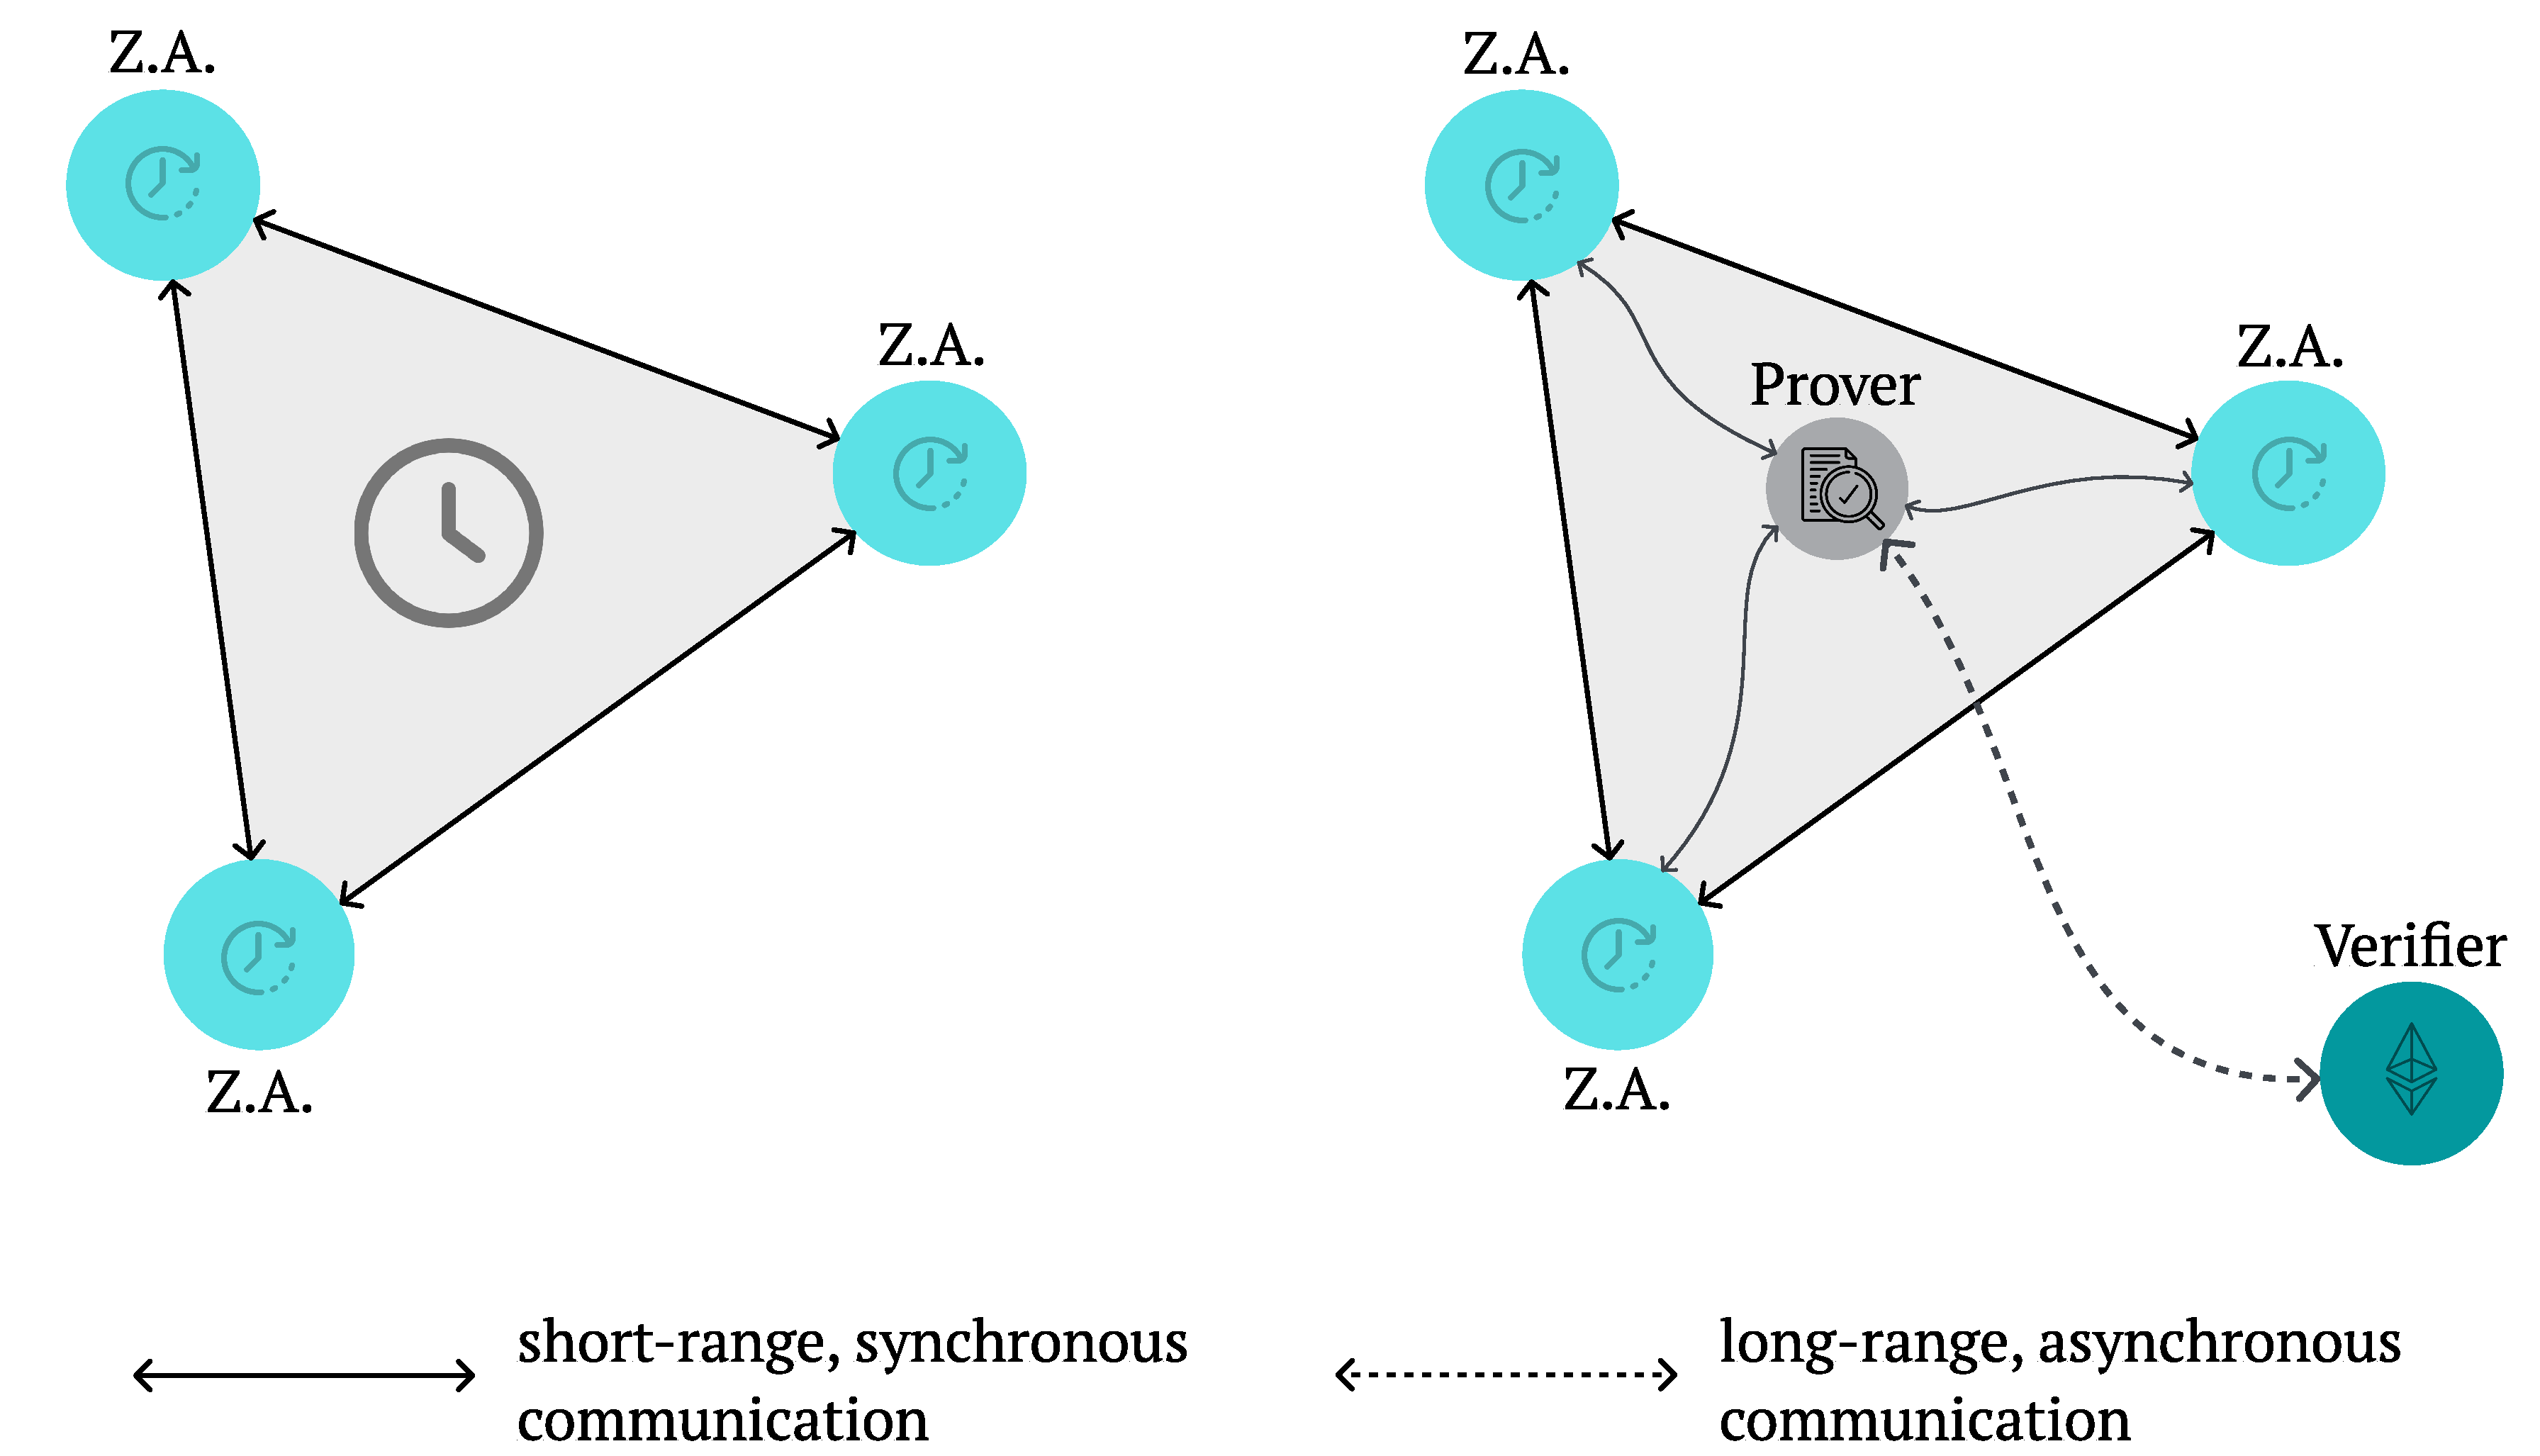
\includegraphics[width=0.9\textwidth]{trustless-pol.pdf}
    \caption{The FOAM protocol for dynamic and decentralized \pol{} \cite{foam-white-paper}.}
    \label{fig:trustless-pol}
    \end{center}
\end{figure}

\newpage

This chapter illustrated the evolution of \pol{} protocols, starting from centralized and trusted solutions and advancing towards decentralized and infrastructure-independent approaches. The distribution of trust has driven the development of modern protocols, culminating in the need for decentralized time synchronization, to make trustless witnesses collectively agree on attesting to the nearby presence of a prover. The FOAM protocol is the ultimate inspiration for the work developed further in this thesis. The processes of zone establishment, spatio-temporal synchronization, and decentralized witnessing consensus will be explored as in FOAM, but taking advantage of WiFi-based mesh networking, for the short-range exchange of information, and by employing a permissionless consensus mechanism, aligned with the concepts introduced in Sections~\ref{sec:background-wireless-mesh-networks}~and~\ref{sec:background-permissionless-consensus}.